% answers.tex —— 1977 年·宁夏卷 · 参考答案与详细解析片段
% 由 tools/generate_projects.py 依来源总账自 1977/1977_数学真题_宁夏_试题.md + 1977/1977_数学真题_宁夏_解析正文.md + 1977/1977_数学真题_宁夏_答案要点.md 生成，勿手改（改源 MD 后重跑）


\begin{gktip}
固定源《宁夏1977年高考数学试题解》是题面与解答连续出现的扫描材料。下文逐题对照源解答并独立复算关键结论；题面记号 $\operatorname{Sin}$、$\operatorname{Cos}$、$\operatorname{tg}$、$\operatorname{Lg}$ 在解析中分别按 $\sin$、$\cos$、$\tan$、$\lg$ 计算。源解答存在若干排印笔误（不影响结论），已在第 9、12、14、15 题与附加题解析处以「源注」说明；题面唯一的排印问题（附加题 2(1) 的括号方向）已在试题卷留注。
\end{gktip}

\begin{answer}
\gksolhead{1}{}

\textbf{题目}（文科 6 分，理科 5 分）：

\Needspace{5\baselineskip}
计算

\nopagebreak[4]
\[
\left(2\frac79\right)^{\frac12}+3^{-2}-\left(\frac13\right)^0.
\]

\Needspace{4\baselineskip}
\textbf{解析}

\nopagebreak[4]
\[
\left(2\frac79\right)^{\frac12}
=\left(\frac{25}{9}\right)^{\frac12}
=\frac53,
\qquad
3^{-2}=\frac19,
\qquad
\left(\frac13\right)^0=1,
\]

\Needspace{5\baselineskip}
故

\nopagebreak[4]
\[
\left(2\frac79\right)^{\frac12}+3^{-2}-\left(\frac13\right)^0
=\frac53+\frac19-1
=\frac{15+1-9}{9}
=\frac79.
\]

\gkanswer{答案：$\dfrac79$。}

\end{answer}
\begin{answer}
\gksolhead{2}{}

\textbf{题目}（文科 6 分，理科 5 分）：

\Needspace{5\baselineskip}
化简：

\nopagebreak[4]
\[
\sqrt{12}-\sqrt{48}-3\sqrt3.
\]

\Needspace{4\baselineskip}
\textbf{解析}

\nopagebreak[4]
\[
\sqrt{12}-\sqrt{48}-3\sqrt3
=2\sqrt3-4\sqrt3-3\sqrt3
=-5\sqrt3.
\]

\gkanswer{答案：$-5\sqrt3$。}

\end{answer}
\begin{answer}
\gksolhead{3}{}

\textbf{题目}（文科 6 分，理科 5 分）：

\Needspace{5\baselineskip}
分解因式：

\nopagebreak[4]
\[
mx^2+2mxy+my^2.
\]

\Needspace{4\baselineskip}
\textbf{解析}

\nopagebreak[4]
\[
mx^2+2mxy+my^2
=m\left(x^2+2xy+y^2\right)
=m(x+y)^2.
\]

\gkanswer{答案：$m(x+y)^2$。}

\end{answer}
\begin{answer}
\gksolhead{4}{}

\textbf{题目}（文科 6 分，理科 5 分）：

\Needspace{5\baselineskip}
解方程：

\nopagebreak[4]
\[
2x^2-3x+1=0.
\]

\Needspace{4\baselineskip}
\textbf{解析}

\nopagebreak[4]
\[
2x^2-3x+1=(x-1)(2x-1)=0,
\]

故 $x_1=1$，$x_2=\dfrac12$。

\gkanswer{答案：$x_1=1$，$x_2=\dfrac12$。}

\end{answer}
\begin{answer}
\gksolhead{5}{}

\textbf{题目}（文科 6 分，理科 5 分）：

已知 $\operatorname{Sin}\alpha=\dfrac35$（$\alpha$ 是锐角），求：

（1） $\operatorname{Cos}\alpha$；

（2） $\operatorname{tg}\alpha$。

\Needspace{4\baselineskip}
\textbf{解析}

已知 $\sin\alpha=\dfrac35$，且 $\alpha$ 为锐角。

\gksubpart{（1）}

\nopagebreak[4]
\[
\cos\alpha=\sqrt{1-\sin^2\alpha}
=\sqrt{1-\left(\frac35\right)^2}
=\frac45.
\]

\gksubpart{（2）}

\nopagebreak[4]
\[
\tan\alpha=\frac{\sin\alpha}{\cos\alpha}
=\dfrac{3/5}{4/5}
=\frac34.
\]

\gkanswer{答案（1）：$\dfrac45$。}

\gkanswer{答案（2）：$\dfrac34$。}

\end{answer}
\begin{answer}
\gksolhead{6}{}

\textbf{题目}（文科 6 分，理科 5 分）：

\Needspace{5\baselineskip}
不查表求：

\nopagebreak[4]
\[
\operatorname{Lg}8+\operatorname{Lg}125-\operatorname{Lg}1.
\]

\Needspace{4\baselineskip}
\textbf{解析}

\nopagebreak[4]
\[
\begin{aligned}
\operatorname{Lg}8+\operatorname{Lg}125-\operatorname{Lg}1
&=3\lg2+3\lg5-0\\
&=3(\lg2+\lg5)=3\lg10=3.
\end{aligned}
\]

\gkanswer{答案：$3$。}

\end{answer}
\begin{answer}
\gksolhead{7}{}

\textbf{题目}（文科 6 分，理科 5 分）：

求经过点 $(4,-4)$ 和原点的直线方程。

\Needspace{4\baselineskip}
\textbf{解析}

\Needspace{5\baselineskip}
设原点为 $O(0,0)$，已知点为 $P(4,-4)$，则直线斜率

\nopagebreak[4]
\[
k=\frac{-4-0}{4-0}=-1,
\]

\Needspace{5\baselineskip}
直线经过原点，故所求直线方程为

\nopagebreak[4]
\[
y=-x.
\]

\gkanswer{答案：$y=-x$。}

\end{answer}
\begin{answer}
\gksolhead{8}{}

\textbf{题目}（文科 6 分，理科 5 分）：

解不等式：$(x+1)(x-2)<0$。

\Needspace{4\baselineskip}
\textbf{解析}

\Needspace{5\baselineskip}
由 $(x+1)(x-2)<0$ 知两因式异号，分为两个不等式组：

\nopagebreak[4]
\[
\text{（I）}\begin{cases}x+1>0,\\ x-2<0,\end{cases}
\qquad
\text{（II）}\begin{cases}x+1<0,\\ x-2>0.\end{cases}
\]

不等式组（I）的解为 $-1<x<2$；不等式组（II）中两不等式不能同时成立，无解。故原不等式的解为 $-1<x<2$。

\gkanswer{答案：$-1<x<2$。}

\end{answer}
\begin{answer}
\gksolhead{9}{}

\textbf{题目}（文科 6 分，理科 5 分）：

\Needspace{5\baselineskip}
求

\nopagebreak[4]
\[
\frac12+\frac14+\frac18+\frac1{16}+\cdots+\frac{1}{2^{10}}.
\]

\Needspace{4\baselineskip}
\textbf{解析}

\Needspace{5\baselineskip}
这是首项为 $\dfrac12$、公比为 $\dfrac12$ 的等比数列前 10 项和，由求和公式

\nopagebreak[4]
\[
\begin{aligned}
\frac12+\frac14+\frac18+\frac1{16}+\cdots+\frac1{2^{10}}
&=\frac{\frac12\left[1-\left(\frac12\right)^{10}\right]}{1-\frac12}\\
&=1-\frac1{2^{10}}
=\frac{2^{10}-1}{2^{10}}
=\frac{1023}{1024}.
\end{aligned}
\]

\begin{gktip}
\textbf{源注}：源解答在复述题面时把第四项印作「$\frac1{10}$」，按题面应为 $\frac1{16}$；求和过程与结论均按题面进行，不受影响。
\end{gktip}

\gkanswer{答案：$\dfrac{1023}{1024}$。}

\end{answer}
\begin{answer}
\gksolhead{10}{}

\textbf{题目}（文科 6 分，理科 5 分）：

已知：在 $\triangle ABC$ 中，$\angle B=60^\circ$，$AD\perp BC$，$AD=3$，$AC=5$。求：$BC$，$AB$。
\nopagebreak[4]
\begin{center}% 1977 年宁夏卷第 10 题：三角形 ABC（A 在上方），AD 为 BC 边上的垂线，D 为垂足（按源卷第 2 页布局）
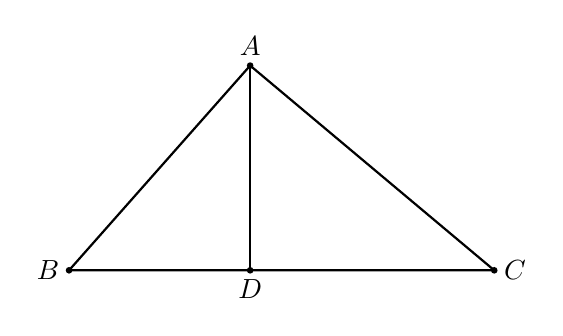
\begin{tikzpicture}[scale=1.0]
  \coordinate (A) at (2.3,2.6);
  \coordinate (B) at (0,0);
  \coordinate (C) at (5.4,0);
  \coordinate (D) at (2.3,0);
  \draw[thick] (B)--(C)--(A)--cycle;
  \draw[thick] (A)--(D);
  \fill (A) circle (1.2pt) node[above] {$A$};
  \fill (B) circle (1.2pt) node[left] {$B$};
  \fill (C) circle (1.2pt) node[right] {$C$};
  \fill (D) circle (1.2pt) node[below] {$D$};
\end{tikzpicture}
\end{center}
\nopagebreak[4]
\Needspace{4\baselineskip}
\textbf{解析}
\nopagebreak[4]
\begin{center}% 1977 年宁夏卷第 10 题：三角形 ABC（A 在上方），AD 为 BC 边上的垂线，D 为垂足（按源卷第 2 页布局）
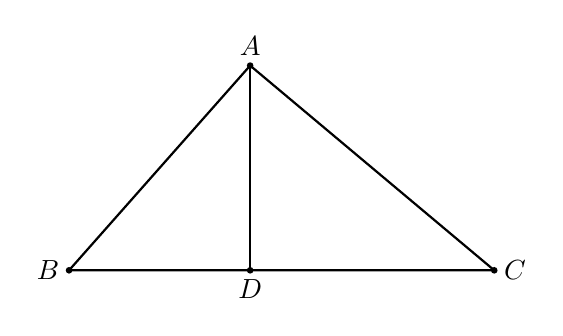
\begin{tikzpicture}[scale=1.0]
  \coordinate (A) at (2.3,2.6);
  \coordinate (B) at (0,0);
  \coordinate (C) at (5.4,0);
  \coordinate (D) at (2.3,0);
  \draw[thick] (B)--(C)--(A)--cycle;
  \draw[thick] (A)--(D);
  \fill (A) circle (1.2pt) node[above] {$A$};
  \fill (B) circle (1.2pt) node[left] {$B$};
  \fill (C) circle (1.2pt) node[right] {$C$};
  \fill (D) circle (1.2pt) node[below] {$D$};
\end{tikzpicture}
\end{center}
\nopagebreak[4]
\Needspace{5\baselineskip}
在 $\triangle ABD$ 中，$\angle ADB=90^\circ$，$\angle B=60^\circ$，$AD=3$，故

\nopagebreak[4]
\[
BD=\frac{AD}{\tan60^\circ}=\frac{3}{\sqrt3}=\sqrt3,
\qquad
AB=\sqrt{AD^2+BD^2}=\sqrt{9+3}=2\sqrt3.
\]

\Needspace{5\baselineskip}
在 $\triangle ACD$ 中，$\angle ADC=90^\circ$，由勾股定理

\nopagebreak[4]
\[
DC=\sqrt{AC^2-AD^2}=\sqrt{25-9}=4,
\]

\Needspace{5\baselineskip}
所以

\nopagebreak[4]
\[
BC=BD+DC=\sqrt3+4.
\]

\gkanswer{答案：$BC=4+\sqrt3$，$AB=2\sqrt3$。}

\end{answer}
\begin{answer}
\gksolhead{11}{}

\textbf{题目}（文科 14 分，理科 12 分）：

在 $\triangle ABC$ 中，已知 $a=\sqrt2$，$A=45^\circ$，$B=60^\circ$，求 $C$、$b$、$c$ 及面积 $\triangle$。
\nopagebreak[4]
\begin{center}% 1977 年宁夏卷第 11 题：三角形 ABC（C 在上方），三边分别标注 a（BC 边）、b（CA 边）、c（AB 边）（按源卷第 2 页布局）
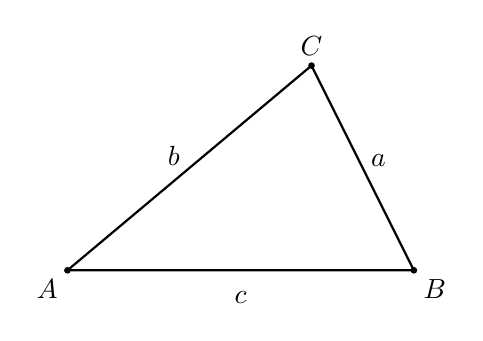
\begin{tikzpicture}[scale=1.0]
  \coordinate (A) at (0,0);
  \coordinate (B) at (4.4,0);
  \coordinate (C) at (3.1,2.6);
  \draw[thick] (A)--(B)--(C)--cycle;
  \fill (A) circle (1.2pt) node[below left] {$A$};
  \fill (B) circle (1.2pt) node[below right] {$B$};
  \fill (C) circle (1.2pt) node[above] {$C$};
  \node at (1.35,1.45) {$b$};
  \node at (3.95,1.4) {$a$};
  \node at (2.2,-0.35) {$c$};
\end{tikzpicture}
\end{center}
\nopagebreak[4]
\Needspace{4\baselineskip}
\textbf{解析}
\nopagebreak[4]
\begin{center}% 1977 年宁夏卷第 11 题：三角形 ABC（C 在上方），三边分别标注 a（BC 边）、b（CA 边）、c（AB 边）（按源卷第 2 页布局）
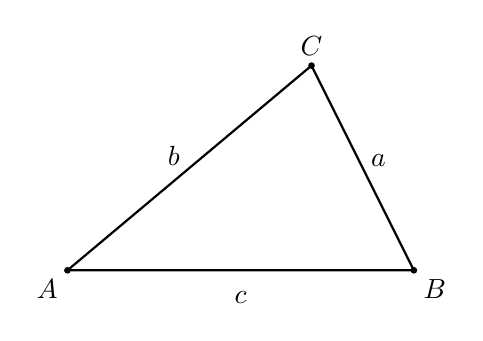
\begin{tikzpicture}[scale=1.0]
  \coordinate (A) at (0,0);
  \coordinate (B) at (4.4,0);
  \coordinate (C) at (3.1,2.6);
  \draw[thick] (A)--(B)--(C)--cycle;
  \fill (A) circle (1.2pt) node[below left] {$A$};
  \fill (B) circle (1.2pt) node[below right] {$B$};
  \fill (C) circle (1.2pt) node[above] {$C$};
  \node at (1.35,1.45) {$b$};
  \node at (3.95,1.4) {$a$};
  \node at (2.2,-0.35) {$c$};
\end{tikzpicture}
\end{center}
\nopagebreak[4]
\Needspace{5\baselineskip}
由三角形内角和，

\nopagebreak[4]
\[
C=180^\circ-(A+B)=180^\circ-105^\circ=75^\circ.
\]

\Needspace{5\baselineskip}
由正弦定理，

\nopagebreak[4]
\[
b=\frac{a\sin B}{\sin A}
=\frac{\sqrt2\sin60^\circ}{\sin45^\circ}
=\frac{\sqrt2\cdot\frac{\sqrt3}{2}}{\frac{\sqrt2}{2}}
=\sqrt3,
\]

\nopagebreak[4]
\[
\begin{aligned}
c&=\frac{a\sin C}{\sin A}
=\frac{\sqrt2\sin75^\circ}{\sin45^\circ}
=2\sin75^\circ\\
&=2\left(\sin30^\circ\cos45^\circ+\cos30^\circ\sin45^\circ\right)
=\frac{\sqrt2+\sqrt6}{2}.
\end{aligned}
\]

\Needspace{5\baselineskip}
面积

\nopagebreak[4]
\[
S=\frac12ab\sin C
=\frac12\cdot\sqrt2\cdot\sqrt3\cdot\frac{\sqrt6+\sqrt2}{4}
=\frac{\sqrt{12}+6}{8}
=\frac{3+\sqrt3}{4}.
\]

\gkanswer{答案：$C=75^\circ$，$b=\sqrt3$，$c=\dfrac{\sqrt2+\sqrt6}{2}$，$S_\triangle=\dfrac{3+\sqrt3}{4}$。}

\end{answer}
\begin{answer}
\gksolhead{12}{}

\textbf{题目}（文科 14 分，理科 12 分）：

求与直线 $x+y=1$ 相切于点 $(2,-1)$，并且圆心在直线 $y=-2x$ 上圆的方程。

\Needspace{4\baselineskip}
\textbf{解析}

\Needspace{5\baselineskip}
\textbf{方法一}：圆心在过切点且垂直于切线的直线上。切线 $x+y=1$ 的斜率为 $-1$，故过切点 $(2,-1)$ 的直径所在直线斜率为 $1$，方程为 $y+1=x-2$。圆心坐标同时满足

\nopagebreak[4]
\[
\begin{cases}
y+1=x-2,\\
y=-2x,
\end{cases}
\]

\Needspace{5\baselineskip}
解得圆心为 $(1,-2)$。由圆心与切点间距离得半径

\nopagebreak[4]
\[
R=\sqrt{(2-1)^2+(-1+2)^2}=\sqrt2.
\]

方法二：设所求圆的方程为 $(x-a)^2+(y-b)^2=R^2$。切点 $(2,-1)$ 在圆上，得 $(2-a)^2+(-1-b)^2=R^2$；圆心在直线 $y=-2x$ 上，得 $b=-2a$；圆心到切线 $x+y-1=0$ 的距离等于半径，得 $\dfrac{|a+b-1|}{\sqrt2}=R$。三式联立解得 $a=1$，$b=-2$，$R=\sqrt2$。

\Needspace{5\baselineskip}
所以所求圆的方程为

\nopagebreak[4]
\[
(x-1)^2+(y+2)^2=2.
\]

\begin{gktip}
\textbf{源注}：源解答方法二中，圆心所到直线的方程印作「$x+y+1=1$」，按切线 $x+y=1$ 应为 $x+y-1=0$（同页距离公式的分子印作 $|a+b-1|$ 亦可佐证），该分子内另多印一处逗号；本文按更正后的直线转写，方法一与方法二结论一致。
\end{gktip}

\gkanswer{答案：$(x-1)^2+(y+2)^2=2$。}

\end{answer}
\begin{answer}
\gksolhead{13}{}

\textbf{题目}（文科 13 分，理科 12 分）：

已知圆内接三角形 $ABC$，$AB$、$BC$ 上的高 $CE$、$AD$ 相交于 $H$，$AD$ 延长线与 $\overset{\frown}{BC}$ 交于 $F$。求证：$HD=FD$。
\nopagebreak[4]
\begin{center}% 1977 年宁夏卷第 13 题：圆内接三角形 ABC，AB、BC 边上的高 CE、AD 相交于 H，
% AD 延长线交弧 BC 于 F，连线 FC 为虚线；角 1 在 B、角 2 在 C、角 3 在 H、角 4 在 F（按源卷第 3 页布局）
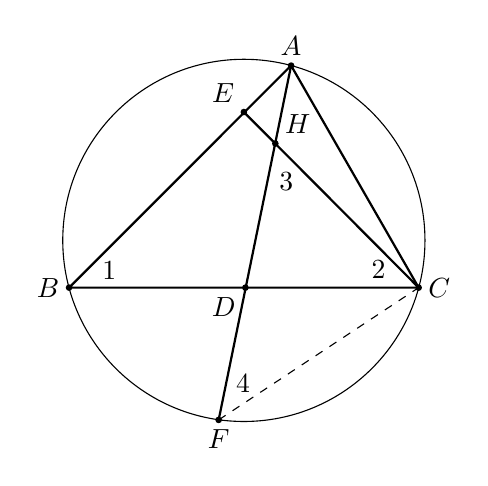
\begin{tikzpicture}[scale=1.0]
  \draw (2.6,2.1) circle (2.3);
  \coordinate (A) at (3.2,4.32);
  \coordinate (B) at (0.38,1.5);
  \coordinate (C) at (4.82,1.5);
  \coordinate (D) at (2.62,1.5);
  \coordinate (E) at (2.6,3.73);
  \coordinate (H) at (3.0,3.33);
  \coordinate (F) at (2.28,-0.18);
  \draw[thick] (A)--(B)--(C)--cycle;
  \draw[thick] (A)--(F);
  \draw[thick] (C)--(E);
  \draw[dashed] (F)--(C);
  \fill (A) circle (1.2pt) node[above] {$A$};
  \fill (B) circle (1.2pt) node[left] {$B$};
  \fill (C) circle (1.2pt) node[right] {$C$};
  \fill (D) circle (1.2pt) node[below left] {$D$};
  \fill (E) circle (1.2pt) node[above left] {$E$};
  \fill (H) circle (1.2pt) node[above right] {$H$};
  \fill (F) circle (1.2pt) node[below] {$F$};
  \node at (0.89,1.72) {$1$};
  \node at (4.31,1.73) {$2$};
  \node at (3.14,2.85) {$3$};
  \node at (2.59,0.28) {$4$};
\end{tikzpicture}
\end{center}
\nopagebreak[4]
\Needspace{4\baselineskip}
\textbf{解析}
\nopagebreak[4]
\begin{center}% 1977 年宁夏卷第 13 题：圆内接三角形 ABC，AB、BC 边上的高 CE、AD 相交于 H，
% AD 延长线交弧 BC 于 F，连线 FC 为虚线；角 1 在 B、角 2 在 C、角 3 在 H、角 4 在 F（按源卷第 3 页布局）
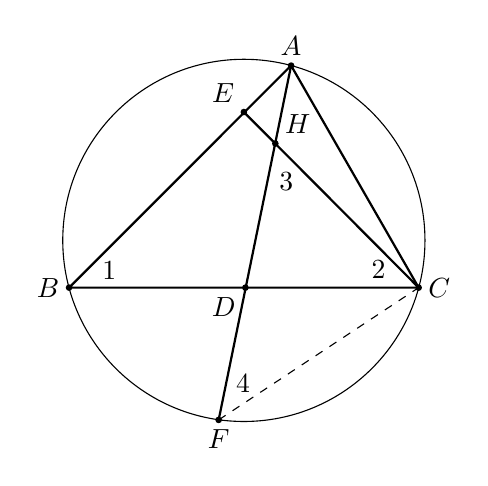
\begin{tikzpicture}[scale=1.0]
  \draw (2.6,2.1) circle (2.3);
  \coordinate (A) at (3.2,4.32);
  \coordinate (B) at (0.38,1.5);
  \coordinate (C) at (4.82,1.5);
  \coordinate (D) at (2.62,1.5);
  \coordinate (E) at (2.6,3.73);
  \coordinate (H) at (3.0,3.33);
  \coordinate (F) at (2.28,-0.18);
  \draw[thick] (A)--(B)--(C)--cycle;
  \draw[thick] (A)--(F);
  \draw[thick] (C)--(E);
  \draw[dashed] (F)--(C);
  \fill (A) circle (1.2pt) node[above] {$A$};
  \fill (B) circle (1.2pt) node[left] {$B$};
  \fill (C) circle (1.2pt) node[right] {$C$};
  \fill (D) circle (1.2pt) node[below left] {$D$};
  \fill (E) circle (1.2pt) node[above left] {$E$};
  \fill (H) circle (1.2pt) node[above right] {$H$};
  \fill (F) circle (1.2pt) node[below] {$F$};
  \node at (0.89,1.72) {$1$};
  \node at (4.31,1.73) {$2$};
  \node at (3.14,2.85) {$3$};
  \node at (2.59,0.28) {$4$};
\end{tikzpicture}
\end{center}
\nopagebreak[4]
\Needspace{5\baselineskip}
记 $\angle1=\angle ABC$（$B$ 处），$\angle2=\angle BCE$（$C$ 处），$\angle3=\angle DHC$（$H$ 处），$\angle4=\angle DFC$（$F$ 处）。由 $CE\perp AB$、$AD\perp BC$，

\nopagebreak[4]
\[
\angle1+\angle2=90^\circ,
\qquad
\angle3+\angle2=90^\circ,
\]

\Needspace{5\baselineskip}
两式相减得

\nopagebreak[4]
\[
\angle1=\angle3.
\]

\Needspace{5\baselineskip}
又 $A$、$B$、$F$、$C$ 四点共圆，$\angle ABC$ 与 $\angle AFC$ 是同弧 $AC$ 上的圆周角，故 $\angle ABC=\angle AFC$；而 $D$ 在 $AF$ 上，$\angle AFC=\angle DFC=\angle4$，于是

\nopagebreak[4]
\[
\angle1=\angle4.
\]

\Needspace{5\baselineskip}
由上两步得 $\angle3=\angle4$。在 $\triangle HDC$ 与 $\triangle FDC$ 中，$\angle HDC=\angle FDC=90^\circ$，$DC$ 为公共边，$\angle DHC=\angle DFC$，故

\nopagebreak[4]
\[
\mathrm{Rt}\,\triangle HDC\cong\mathrm{Rt}\,\triangle FDC,
\]

\Needspace{5\baselineskip}
从而

\nopagebreak[4]
\[
HD=FD.
\]

\gkanswer{答案：见解析版}

\end{answer}
\begin{answer}
\gksolhead{14}{}

\textbf{题目}（文科 13 分，理科 12 分）：

用 $6$ 米长的条形木料做如图的矩形窗框（包括中间的两个横档），问窗框的长、宽尺寸如何选择，窗框的面积最大？
\nopagebreak[4]
\begin{center}% 1977 年宁夏卷第 14 题：矩形窗框（含中间两个横档，分成上下三格），
% 右侧括线标长 x，底部括线标宽 (6-2x)/4（按源卷第 3 页布局）
\begin{tikzpicture}[scale=1.0]
  \draw[thick] (0,0) rectangle (1.7,4.2);
  \draw[thick] (0,1.4) -- (1.7,1.4);
  \draw[thick] (0,2.8) -- (1.7,2.8);
  \draw[thick] (1.95,0) -- (2.15,0) -- (2.15,4.2) -- (1.95,4.2);
  \node at (2.6,2.1) {$x$};
  \draw[thick] (0,-0.25) -- (0,-0.45) -- (1.7,-0.45) -- (1.7,-0.25);
  \node at (0.85,-0.95) {$\dfrac{6-2x}{4}$};
\end{tikzpicture}
\end{center}
\nopagebreak[4]
\Needspace{4\baselineskip}
\textbf{解析}
\nopagebreak[4]
\begin{center}% 1977 年宁夏卷第 14 题：矩形窗框（含中间两个横档，分成上下三格），
% 右侧括线标长 x，底部括线标宽 (6-2x)/4（按源卷第 3 页布局）
\begin{tikzpicture}[scale=1.0]
  \draw[thick] (0,0) rectangle (1.7,4.2);
  \draw[thick] (0,1.4) -- (1.7,1.4);
  \draw[thick] (0,2.8) -- (1.7,2.8);
  \draw[thick] (1.95,0) -- (2.15,0) -- (2.15,4.2) -- (1.95,4.2);
  \node at (2.6,2.1) {$x$};
  \draw[thick] (0,-0.25) -- (0,-0.45) -- (1.7,-0.45) -- (1.7,-0.25);
  \node at (0.85,-0.95) {$\dfrac{6-2x}{4}$};
\end{tikzpicture}
\end{center}
\nopagebreak[4]
\Needspace{5\baselineskip}
设窗框的长为 $x$ 米。木料总长用于两条长边与四条宽边（上下两边加两个横档），故宽为 $\dfrac{6-2x}{4}=\dfrac{3-x}{2}$ 米，面积

\nopagebreak[4]
\[
S=x\cdot\frac{3-x}{2}
=-\frac12x^2+\frac32x
=-\frac12\left(x-\frac32\right)^2+\frac98.
\]

当 $x=\dfrac32$ 时 $S$ 取最大值 $\dfrac98$，此时宽为 $\dfrac{3-\frac32}{2}=\dfrac34$ 米。即窗框的长为 $\dfrac32$ 米、宽为 $\dfrac34$ 米时，窗框面积最大。

\begin{gktip}
\textbf{源注}：源解答展开式的一次项系数印作「$+\frac23x$」，按 $S=x\cdot\frac{3-x}{2}$ 展开应为 $+\frac32x$；其后配方 $-\frac12\left(x-\frac32\right)^2+\frac98$ 与答句（长 $\frac32$ 米、宽 $\frac34$ 米）均按 $\frac32$ 成立，系排印笔误，本文按 $\frac32$ 计算。
\end{gktip}

\gkanswer{答案：长 $\dfrac32$ 米、宽 $\dfrac34$ 米，最大面积 $\dfrac98$ 平方米。}

\end{answer}
\begin{answer}
\gksolhead{15}{}

\textbf{题目}（理科 14 分，文科不作）：

一大正六边形内接一个小正六边形，小正六边形各顶点分大正六边形各边成 $m$、$n$ 两段。

（1） 求小正六边形的面积 $S_{\text{\text{小}}}$；

（2） 证明 $4S_{\text{\text{小}}}\ge 3S_{\text{\text{大}}}$（$S_{\text{\text{大}}}$ 表示大正六边形的面积）。
\nopagebreak[4]
\begin{center}% 1977 年宁夏卷第 15 题：平顶大正六边形 ABCDEF，各边上的分点 A'、B'、C'、D'、E'、F'
% 连成内接小正六边形；AA' 段标 m，A'B 段标 n（按源卷第 4 页布局）
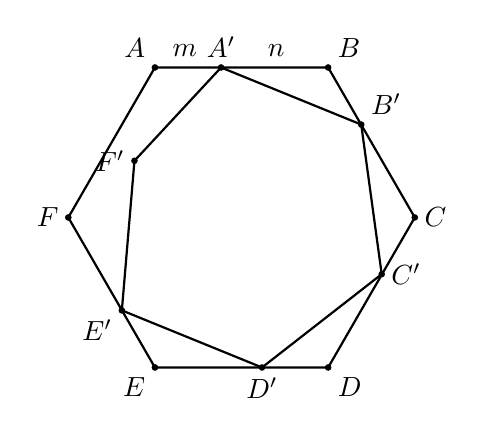
\begin{tikzpicture}[scale=1.0]
  \coordinate (A) at (-1.1,1.905);
  \coordinate (B) at (1.1,1.905);
  \coordinate (C) at (2.2,0);
  \coordinate (D) at (1.1,-1.905);
  \coordinate (E) at (-1.1,-1.905);
  \coordinate (F) at (-2.2,0);
  \coordinate (Ap) at (-0.26,1.905);
  \coordinate (Bp) at (1.52,1.18);
  \coordinate (Cp) at (1.78,-0.72);
  \coordinate (Dp) at (0.26,-1.905);
  \coordinate (Ep) at (-1.52,-1.18);
  \coordinate (Fp) at (-1.36,0.72);
  \draw[thick] (A)--(B)--(C)--(D)--(E)--(F)--cycle;
  \draw[thick] (Ap)--(Bp)--(Cp)--(Dp)--(Ep)--(Fp)--cycle;
  \fill (A) circle (1.2pt) node[above left] {$A$};
  \fill (B) circle (1.2pt) node[above right] {$B$};
  \fill (C) circle (1.2pt) node[right] {$C$};
  \fill (D) circle (1.2pt) node[below right] {$D$};
  \fill (E) circle (1.2pt) node[below left] {$E$};
  \fill (F) circle (1.2pt) node[left] {$F$};
  \fill (Ap) circle (1.2pt) node[above] {$A'$};
  \fill (Bp) circle (1.2pt) node[above right] {$B'$};
  \fill (Cp) circle (1.2pt) node[right] {$C'$};
  \fill (Dp) circle (1.2pt) node[below] {$D'$};
  \fill (Ep) circle (1.2pt) node[below left] {$E'$};
  \fill (Fp) circle (1.2pt) node[left] {$F'$};
  \node at (-0.72,2.12) {$m$};
  \node at (0.44,2.12) {$n$};
\end{tikzpicture}
\end{center}
\nopagebreak[4]
\begin{gktip}
\textbf{附加题}（原卷注明：满分 20 分，在 100 分之外，计入总分）
\end{gktip}

\textbf{附加题 1．} 已知 $\operatorname{Cos}\alpha+\operatorname{Sin}\alpha=\dfrac1{\sqrt2}$。试求：

（1） $\operatorname{Sin}^4\alpha+\operatorname{Cos}^4\alpha$；

（2） $\operatorname{Sin}^5\alpha+\operatorname{Cos}^5\alpha$。

\textbf{附加题 2．}

（1） 若 $a_i>0$（$i=1,2,\cdots,n$），证明：$\sum_{i=1}^{n}a_i\cdot\sum_{i=1}^{n}\frac1{a_i}\ge n^2$；

（2） 若 $f(x)$ 在 $[0,1]$ 上连续，且 $f(x)>0$，证明 $\int_0^1 f(x)\,dx\int_0^1\frac{dx}{f(x)}\ge 1$。

\begin{gktip}
\textbf{源注}：附加题 2(1) 题干中「$a_i>0$」后的括号在原卷排印为闭括号（原样为「$a_i>0$）$i=1,2,\cdots,n$）」），本库按开括号理解转录，未增删题干内容。
\end{gktip}

\Needspace{4\baselineskip}
\textbf{解析}
\nopagebreak[4]
\begin{center}% 1977 年宁夏卷第 15 题：平顶大正六边形 ABCDEF，各边上的分点 A'、B'、C'、D'、E'、F'
% 连成内接小正六边形；AA' 段标 m，A'B 段标 n（按源卷第 4 页布局）
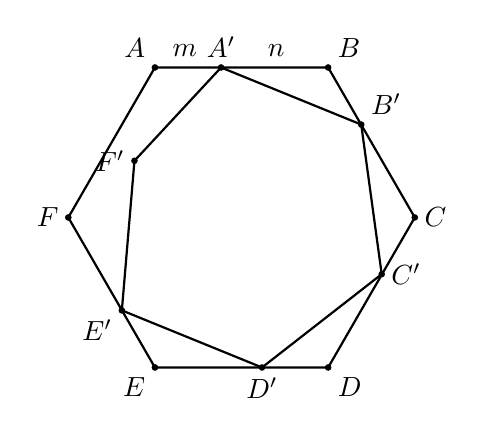
\begin{tikzpicture}[scale=1.0]
  \coordinate (A) at (-1.1,1.905);
  \coordinate (B) at (1.1,1.905);
  \coordinate (C) at (2.2,0);
  \coordinate (D) at (1.1,-1.905);
  \coordinate (E) at (-1.1,-1.905);
  \coordinate (F) at (-2.2,0);
  \coordinate (Ap) at (-0.26,1.905);
  \coordinate (Bp) at (1.52,1.18);
  \coordinate (Cp) at (1.78,-0.72);
  \coordinate (Dp) at (0.26,-1.905);
  \coordinate (Ep) at (-1.52,-1.18);
  \coordinate (Fp) at (-1.36,0.72);
  \draw[thick] (A)--(B)--(C)--(D)--(E)--(F)--cycle;
  \draw[thick] (Ap)--(Bp)--(Cp)--(Dp)--(Ep)--(Fp)--cycle;
  \fill (A) circle (1.2pt) node[above left] {$A$};
  \fill (B) circle (1.2pt) node[above right] {$B$};
  \fill (C) circle (1.2pt) node[right] {$C$};
  \fill (D) circle (1.2pt) node[below right] {$D$};
  \fill (E) circle (1.2pt) node[below left] {$E$};
  \fill (F) circle (1.2pt) node[left] {$F$};
  \fill (Ap) circle (1.2pt) node[above] {$A'$};
  \fill (Bp) circle (1.2pt) node[above right] {$B'$};
  \fill (Cp) circle (1.2pt) node[right] {$C'$};
  \fill (Dp) circle (1.2pt) node[below] {$D'$};
  \fill (Ep) circle (1.2pt) node[below left] {$E'$};
  \fill (Fp) circle (1.2pt) node[left] {$F'$};
  \node at (-0.72,2.12) {$m$};
  \node at (0.44,2.12) {$n$};
\end{tikzpicture}
\end{center}
\nopagebreak[4]
\gksubpart{（1）}

\Needspace{5\baselineskip}
由图可知 $A'B=n$，$BB'=m$，正六边形内角 $\angle B=120^\circ$。在 $\triangle A'BB'$ 中，由余弦定理

\nopagebreak[4]
\[
A'B'^2=m^2+n^2-2mn\cos120^\circ=m^2+n^2+mn.
\]

\Needspace{5\baselineskip}
小正六边形由 6 个边长为 $A'B'$ 的正三角形组成，故

\nopagebreak[4]
\[
S_{\text{\text{小}}}=6\cdot\frac{\sqrt3}{4}A'B'^2
=\frac{3\sqrt3}{2}\left(m^2+n^2+mn\right).
\]

\gksubpart{（2）}

\Needspace{5\baselineskip}
大正六边形边长 $AB=m+n$，故

\nopagebreak[4]
\[
3S_{\text{\text{大}}}=3\cdot\frac{3\sqrt3}{2}(m+n)^2
=\frac{9\sqrt3}{2}(m+n)^2.
\]

\Needspace{5\baselineskip}
作差配方：

\nopagebreak[4]
\[
\begin{aligned}
4S_{\text{\text{小}}}-3S_{\text{\text{大}}}
&=6\sqrt3\left(m^2+n^2+mn\right)-\frac{9\sqrt3}{2}(m+n)^2\\
&=\frac{3\sqrt3}{2}\left[4\left(m^2+n^2+mn\right)-3(m+n)^2\right]\\
&=\frac{3\sqrt3}{2}\left(m^2+n^2-2mn\right)
=\frac{3\sqrt3}{2}(m-n)^2\ge0.
\end{aligned}
\]

所以 $4S_{\text{\text{小}}}\ge 3S_{\text{\text{大}}}$，当且仅当 $m=n$ 时取等号。

\begin{gktip}
\textbf{源注}：源解答按均值不等式 $mn\le\left(\frac{m+n}{2}\right)^2$ 放缩时，中间一步不等号印作「$\le$」，按不等号方向应为「$\ge$」；本文改用作差配方直接证明，结论与源解答一致。
\end{gktip}

\textbf{附加题 1}

\Needspace{4\baselineskip}
\textbf{解析}

\Needspace{5\baselineskip}
记已知等式为 $\cos\alpha+\sin\alpha=\dfrac1{\sqrt2}$，两边平方：

\nopagebreak[4]
\[
1+2\sin\alpha\cos\alpha=\frac12,
\qquad
\sin\alpha\cos\alpha=-\frac14.
\]

\gksubpart{（1）}

\nopagebreak[4]
\[
\begin{aligned}
\sin^4\alpha+\cos^4\alpha
&=\left(\sin^2\alpha+\cos^2\alpha\right)^2-2\sin^2\alpha\cos^2\alpha\\
&=1-2\left(-\frac14\right)^2
=\frac78.
\end{aligned}
\]

\gksubpart{（2）}

\Needspace{5\baselineskip}
先化简：

\nopagebreak[4]
\[
\begin{aligned}
\sin^5\alpha+\cos^5\alpha
&=\left(\sin^4\alpha+\cos^4\alpha\right)(\sin\alpha+\cos\alpha)\\
&\quad-\sin\alpha\cos\alpha\left(\sin^3\alpha+\cos^3\alpha\right)\\
&=(\sin\alpha+\cos\alpha)\bigl[\left(\sin^4\alpha+\cos^4\alpha\right)\\
&\quad-\sin\alpha\cos\alpha(\sin\alpha+\cos\alpha)^2
+3\sin^2\alpha\cos^2\alpha\bigr].
\end{aligned}
\]

\Needspace{5\baselineskip}
代入 $\sin\alpha+\cos\alpha=\dfrac1{\sqrt2}$、$\sin^4\alpha+\cos^4\alpha=\dfrac78$、$\sin\alpha\cos\alpha=-\dfrac14$：

\nopagebreak[4]
\[
\begin{aligned}
\sin^5\alpha+\cos^5\alpha
&=\frac1{\sqrt2}\left[\frac78-\left(-\frac14\right)\times\frac12+3\times\frac1{16}\right]\\
&=\frac1{\sqrt2}\cdot\frac{19}{16}
=\frac{19\sqrt2}{32}.
\end{aligned}
\]

\begin{gktip}
\textbf{源注}：源解答在平方关系处把 $\sin\alpha\cos\alpha$ 排印为「SinαCoa」，漏排一个字母 s，本文按 $\sin\alpha\cos\alpha$ 转写。
\end{gktip}

\textbf{附加题 2}

\Needspace{4\baselineskip}
\textbf{解析}

\gksubpart{（1）}

\Needspace{5\baselineskip}
由 $n$ 个正数的算术平均数不小于几何平均数，

\nopagebreak[4]
\[
\sum_{i=1}^{n}a_i\ge n\sqrt[n]{\prod_{i=1}^{n}a_i},
\qquad
\sum_{i=1}^{n}\frac1{a_i}\ge n\sqrt[n]{\frac1{\prod_{i=1}^{n}a_i}},
\]

\Needspace{5\baselineskip}
其中 $\prod_{i=1}^{n}a_i$ 表示 $a_1a_2\cdots a_n$。两式相乘，

\nopagebreak[4]
\[
\sum_{i=1}^{n}a_i\cdot\sum_{i=1}^{n}\frac1{a_i}
\ge n^2\sqrt[n]{\frac{\prod_{i=1}^{n}a_i}{\prod_{i=1}^{n}a_i}}
=n^2.
\]

\gksubpart{（2）}

\Needspace{5\baselineskip}
在 $[0,1]$ 内等距插入分点 $x_i=\dfrac{i}{n}$（$i=0,1,\cdots,n$），则 $\Delta x_i=\dfrac1n$。由定积分定义，

\nopagebreak[4]
\[
\int_0^1 f(x)\,dx=\lim_{n\to\infty}\frac1n\sum_{i=1}^{n}f(x_i),
\]

\nopagebreak[4]
\[
\int_0^1\frac{dx}{f(x)}=\lim_{n\to\infty}\frac1n\sum_{i=1}^{n}\frac1{f(x_i)}.
\]

\Needspace{5\baselineskip}
由 $f(x_i)>0$ 与均值不等式，

\nopagebreak[4]
\[
\begin{aligned}
\frac1n\sum_{i=1}^{n}f(x_i)
&\ge\sqrt[n]{\prod_{i=1}^{n}f(x_i)},\\
\frac1n\sum_{i=1}^{n}\frac1{f(x_i)}
&\ge\sqrt[n]{\frac1{\prod_{i=1}^{n}f(x_i)}}.
\end{aligned}
\]

\Needspace{5\baselineskip}
两式相乘，对每个 $n$ 都有

\nopagebreak[4]
\[
\left(\frac1n\sum_{i=1}^{n}f(x_i)\right)
\left(\frac1n\sum_{i=1}^{n}\frac1{f(x_i)}\right)
\ge 1.
\]

\Needspace{5\baselineskip}
$f$ 在 $[0,1]$ 上连续保证上式左端两个极限存在，令 $n\to\infty$ 取极限即得

\nopagebreak[4]
\[
\int_0^1 f(x)\,dx\int_0^1\frac{dx}{f(x)}\ge 1.
\]

\begin{gktip}
\textbf{源注}：源解答第二个积分定义式末端的极限记号印作「Jim」，系「Lim」之误，本文按 $\lim$ 转写。
\end{gktip}

\gkanswer{答案（1）：$S_{\text{\text{小}}}=\dfrac{3\sqrt3}{2}\left(m^2+n^2+mn\right)$。}

\gkanswer{答案（2）：见解析版}

\end{answer}